\subsection{Extracted plates}
The extracted plate is also rotated according on contour data. If the contour fails to be detected properly, this also fails. Figure \ref{fig:ExtractedResult1}, \ref{fig:ExtractedResult2}, \ref{fig:ExtractedResult3}, and \ref{fig:ExtractedResult4} have some experimental results of the extracted plates.

\begin{figure}
\begin{subfigure}{0.5\textwidth}
    \centering
    
\includegraphics[width=0.9\linewidth]{./img/experiment/stage.12/00-good}
    \caption{Original Plate}
\end{subfigure}
\begin{subfigure}{0.5\textwidth}
    \centering
    
\includegraphics[width=0.9\linewidth]{./img/experiment/stage.13/00-00-good}
    \caption{Sole extracted image}
\end{subfigure}
\caption{Extracted parts of a good estimation}
\label{fig:ExtractedResult1}
\end{figure}

\begin{figure}
\begin{subfigure}{0.33\textwidth}
    \centering
    
\includegraphics[width=0.9\linewidth]{./img/experiment/stage.12/00-good3}
    \caption{Original Plate}
\end{subfigure}
\begin{subfigure}{0.33\textwidth}
    \centering
    
\includegraphics[width=0.9\linewidth]{./img/experiment/stage.13/00-00-good3}
    \caption{First extracted image}    
\end{subfigure}
\begin{subfigure}{0.33\textwidth}
    \centering
    
\includegraphics[width=0.9\linewidth]{./img/experiment/stage.13/01-00-good3}
    \caption{Second extracted image}
\end{subfigure}
\caption{Extracted parts of another good estimation}
\label{fig:ExtractedResult2}
\end{figure}


\begin{figure}
\begin{subfigure}{0.33\textwidth}
    \centering
    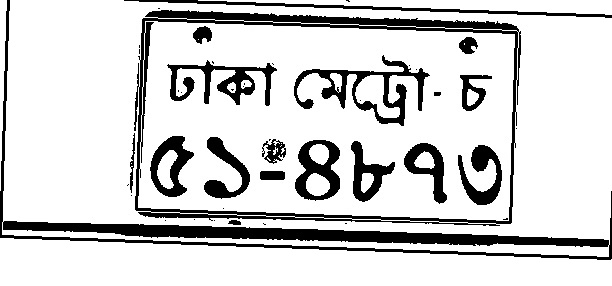
\includegraphics[width=0.9\linewidth]{./img/experiment/stage.12/00-angle}
    \caption{Original Plate}
\end{subfigure}
\begin{subfigure}{0.33\textwidth}
    \centering
    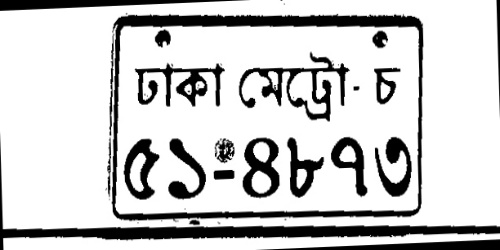
\includegraphics[width=0.9\linewidth]{./img/experiment/stage.13/00-00-angle}
    \caption{First extracted image}
\end{subfigure}
\begin{subfigure}{0.33\textwidth}
    \centering
    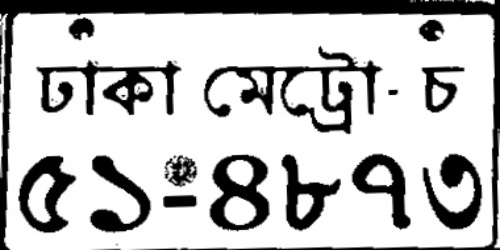
\includegraphics[width=0.9\linewidth]{./img/experiment/stage.13/01-00-angle}
    \caption{Second extracted image}
\end{subfigure}
\caption{Extracted parts of angled plate}
\label{fig:ExtractedResult3}
\end{figure}


\begin{figure}
\begin{subfigure}{0.33\textwidth}
    \centering
    
\includegraphics[width=0.9\linewidth]{./img/experiment/stage.12/02-private}
    \caption{Original Plate}
\end{subfigure}
\begin{subfigure}{0.33\textwidth}
    \centering
    
\includegraphics[width=0.9\linewidth]{./img/experiment/stage.13/00-02-private}
    \caption{First extracted image}
\end{subfigure}
\begin{subfigure}{0.33\textwidth}
    \centering
    
\includegraphics[width=0.9\linewidth]{./img/experiment/stage.13/01-02-private}
    \caption{Second extracted image}
\end{subfigure}
\caption{Extracted parts of a private plate}
\label{fig:ExtractedResult4}
\end{figure}



